\documentclass[final]{beamer}

\mode<presentation>
{
  \usetheme{hiitposter}
}
%\graphicspath{{imgs/}}
\usepackage{amsmath,amsthm, amssymb,mathrsfs}
\usepackage{color}
\usepackage{times}
\usepackage{subfigure}
\usepackage{bm}
\usepackage{url}
\usepackage[numbers]{natbib}
\usepackage[orientation=portrait,size=a0,scale=1.4,debug]{beamerposter}        
%\usepackage[orientation=portrait,width = 91 ,height = 122 ,scale=1.39,debug]{beamerposter} 
%\setbeamerfont{itemize/enumerate body}{size={\fontsize{25}{31}}}
%\setbeamerfont{itemize/enumerate subbody}{size=\footnotesize}

\graphicspath{{../qNML_images/}}

\def\newblock{\hskip .11em plus .33em minus 3.07em}

\definecolor{DRed}{rgb}{0.8,0.6,0.6}
\definecolor{DGreen}{rgb}{0.6,0.7,0.6}
\definecolor{BRed}{rgb}{0.7,0,0}
\definecolor{BGreen}{rgb}{0,0.7,0}

\newcommand{\myred}[1]{{\color{BRed}#1}}
\newcommand{\mygreen}[1]{{\color{BGreen}#1}}


\newcommand{\heading}[1]{\alert{\large #1}\\}
\definecolor{myPurple}{RGB}{174, 206, 195}
%\definecolor{myPurple}{RGB}{165,206,190}


\usepackage{textpos}
\usepackage{fancybox}
\usepackage{tikz}
\usepackage{mathtools}
\usepackage{empheq}

\theoremstyle{plain}
\newtheorem{assumption}{Assumption}

\definecolor{myblue}{rgb}{.85, .85, 1.0}

%%%%%%%%%%%%%%%%%%%%%%%%%%%%%%%%%%%%%%%%
\newlength\mytemplen
\newsavebox\mytempbox

\makeatletter
\newcommand\mybluebox{%
    \@ifnextchar[%]
       {\@mybluebox}%
       {\@mybluebox[0pt]}}

\def\@mybluebox[#1]{%
    \@ifnextchar[%]
       {\@@mybluebox[#1]}%
       {\@@mybluebox[#1][0pt]}}

\def\@@mybluebox[#1][#2]#3{
    \sbox\mytempbox{#3}%
    \mytemplen\ht\mytempbox
    \advance\mytemplen #1\relax
    \ht\mytempbox\mytemplen
    \mytemplen\dp\mytempbox
    \advance\mytemplen #2\relax
    \dp\mytempbox\mytemplen
    \colorbox{myblue}{\hspace{1em}\usebox{\mytempbox}\hspace{1em}}}

\makeatother
%%%%%%%%%%%%%%%%%%%%%%%%%%%%%%%%%%%%%%%%
\makeatletter
\newcommand\mathcircled[1]{%
  \mathpalette\@mathcircled{#1}%
}
\newcommand\@mathcircled[2]{%
  \tikz[baseline=(math.base)] \node[red,draw,circle,inner sep=1pt] (math) {$\m@th#1#2$};%
}
\makeatother


\title{Quotient Normalized Maximum Likelihood Criterion for Learning Bayesian Network Structures}
\author{Tomi Silander$^1$, Janne Lepp{\"a}-aho$^2$, Elias J{\"a}{\"a}saari$^2$, and Teemu Roos$^2$}
\institute{$^{1}$ NAVER LABS Europe, France \\ 
$^{2}$ HIIT / Department of Computer Science, University of Helsinki, Finland}

\begin{document}
\begin{frame}{}
\vskip-1.0ex

{
\setbeamercolor{block body}{bg=myPurple}
\begin{block}{Abstract}
	\large
  	We introduce an information theoretic criterion for Bayesian network
  	structure learning which we call quotient normalized maximum
	likelihood (qNML). In contrast to the closely related factorized
	normalized maximum likelihood criterion, qNML satisfies the property
	of score equivalence. It is also decomposable and completely free
	of adjustable hyperparameters. For practical computations, we identify
	a remarkably accurate approximation proposed earlier by Szpankowski
	and Weinberger. Experiments on both simulated and real data
	demonstrate that the new criterion leads to parsimonious models with
	good predictive accuracy.
\end{block}
}

\begin{block}{Background: Structure Learning of Bayesian Networks}
\begin{columns}[T]
   \begin{column}{0.3\textwidth} % first column {{{
     \heading{Bayesian Networks}
     \vspace*{12pt}
     \begin{itemize}
     \setlength\itemsep{1em}
     \item Provide a compact way to represent a joint distribution over a random vector $X = (X_1, \ldots , X_d)$. 
     %\item Here, each $X_i$ is a categorical random variable.
     \item Consist of:
     \begin{itemize}
     \item[1.] A Directed acyclic graph $G$ which encodes the dependencies between the components of $X$.
     \item[2.] Parameters $\theta = (\theta_1,\ldots,\theta_d)$, where $\theta_i$ denotes the parameters of the conditional distribution of $X_i$ given its parents $G_i$. 
     \end{itemize}
     \item Decomposition: $P(X \mid G, \theta) = \prod_{i=1}^dP(X_i\mid G_i,\theta_i)$
     \end{itemize}     
   \end{column}
  
   \begin{column}{0.005\textwidth}\linethickness{0.3ex} % separator {{{
      \color{myPurple} \line(0,1){450}
   \end{column} % }}}
   
   \begin{column}{0.3\textwidth} % second column {{{
     \heading{Structure Learning}
     \vspace*{12pt}
     \begin{itemize}
     \setlength\itemsep{1em}
     \item[Data:] Each $X_i$ is a categorical variable. We observe $n$ independent samples of $X$ which are collected in a data matrix $D$ of size $n\times d$. 
     \item[Goal:] We consider a \textit{score-based} approach and seek a graph $G$ that maximizes a scoring function which evaluates how well a given graph fits the observed data.
     \item Some scoring functions: BIC, BDeu and fNML. 
   	 \end{itemize}
   \end{column}
  
   \begin{column}{0.005\textwidth}\linethickness{0.3ex} % separator {{{
      \color{myPurple} \line(0,1){450}
   \end{column} % }}}
   \begin{column}{0.3\textwidth}% third column {{{
     \heading{Scoring Functions}
     \begin{itemize}
     
	 \vspace*{12pt}
	 \setlength\itemsep{1em}     
     \item[BDeu] Bayesian marginal likelihood based on Dirichlet priors. Depends on a single 
     hyperparameter $\alpha >0$ called equivalent sample size. 
     \item[BIC] Maximized likelihood with penalty $\frac{k}{2}\log n$, where $k$ is the number of free parameters in the network. 
     \item[fNML] Factorized Normalized Maximum likelihood. Maximized likelihood with penalty defined via \textit{regret} functions.
     \end{itemize}
     
   \end{column} % end of first column }}}
\end{columns}
\end{block}


\begin{block}{Quotient Normalized Maximum Likelihood Criterion}
\begin{columns}[T]
   \begin{column}{0.18\textwidth} % first column {{{
   \heading{Motivation}
   \vspace*{12pt}
   	\textcolor{teal}{BDeu}
	\begin{itemize}	    
    \item Is very sensitive to the choice of the hyperparameter $\alpha$ \cite{cosco.uai07}.
    \item Is not \textit{regular} \cite{Suzuki2017} (can be shown in certain situations to favour too complex models over simpler) 
    \end{itemize}
    \vspace*{12pt}
    \textcolor{teal}{fNML}
	\begin{itemize}	    
    \item Is not score equivalent: the graphs expressing the same independence statements are not scored equally.
    \item Learned structures are often rather complex, which hampers their interpretation.
    \end{itemize}
    
    %\vspace*{12pt} 
	%\textcolor{HIITgreen}{Figure:} Number of parameters as a function of sample size for UCI Breast Cancer  data.     
    
    \end{column}

   \begin{column}{0.18\textwidth}
   \vphantom{\large Motivation}
   \vspace*{12pt} 
    \textcolor{teal}{BIC}
    \begin{itemize}
    \item Appears to
require large sample sizes in order to identify appropriate
structures \cite{cosco.pgm08a,Liu2012}. 
	\end{itemize}  
	
	
	\begin{figure}
  	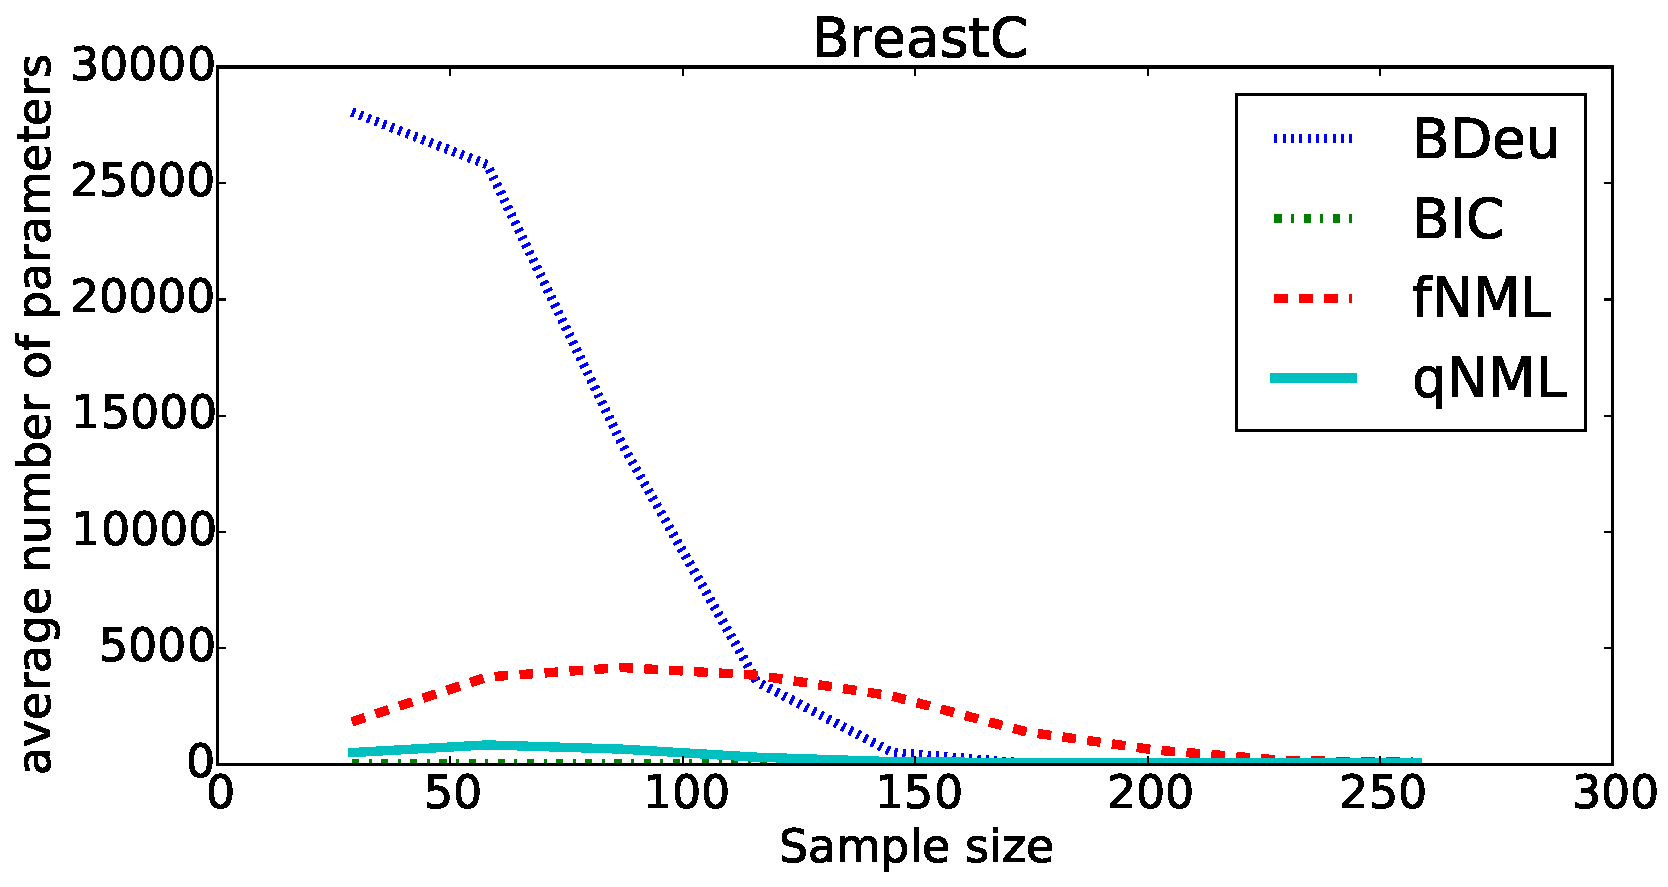
\includegraphics[width=\textwidth]{breast_cancer_npmean.pdf}
  	\caption{Number of parameters as a function of sample size for Breast Cancer (UCI) data.}
  	\end{figure}

   \end{column}
   
   \begin{column}{0.005\textwidth}\linethickness{0.3ex} % separator {{{
      \color{myPurple} \line(0,1){650}
   \end{column} % }}}
   
   \begin{column}{0.3\textwidth} % second column {{{
	\heading{qNML: Definition}
	\vspace*{12pt}
	\begin{itemize}
	\item We would like to choose a model $G$ maximizing	
	\begin{equation}
	P_{NML}(D;G)=\frac{P(D \mid \hat\theta , G)}{\sum_{D'}{P(D' \mid \hat  \theta,G)}},
	\end{equation}where $\hat\theta$ denotes the maximum likelihood parameters.
	\end{itemize}
	
   \end{column}
   
   \begin{column}{0.005\textwidth}\linethickness{0.3ex} % separator {{{
      \color{myPurple} \line(0,1){650}
   \end{column} % }}}
   
   
   \begin{column}{0.25\textwidth}% third column {{{
   
      \heading{qNML: Properties}
   
   \end{column} % end of first column }}}
   % \begin{column}{0.005\textwidth}\linethickness{0.3ex} % separator {{{
   %    \color{myPurple} \line(0,1){600}
   % \end{column} % }}}
   % \begin{column}{0.3\textwidth} % third column {{{
   % \end{column} % end of third column }}}
   
\end{columns}
\end{block}

\begin{block}{Experimental Results}
  \begin{columns}[T]
    \begin{column}{0.35\textwidth}
      \heading{Structure Learning}

    \end{column}
   \begin{column}{0.005\textwidth}\linethickness{0.3ex}
      \color{myPurple} \line(0,1){700}
   \end{column} % }}}
   
    \begin{column}{0.23\textwidth}
    \heading{Prediction}
      
    \end{column}
    
    \begin{column}{0.005\textwidth}\linethickness{0.3ex} % separator {{{
      \color{myPurple} \line(0,1){700}
   \end{column} % }}}
    \begin{column}{0.3\textwidth}
    \heading{Conclusions}

    \end{column}
  \end{columns}
\end{block}

\vskip-1.0ex
\begin{columns}[T]
  \begin{column}{0.63\paperwidth}
\begin{block}{References} %{{{
%\scriptsize
\tiny
{
\bibliographystyle{apalike}
\bibliography{../cosco}
}
\end{block} %}}}
  \end{column}
  \begin{column}{0.33\paperwidth}
\begin{block}{Acknowledgements} %{{{
%\scriptsize
\tiny
{
J.L., E.J. and T.R. were supported by the Academy of Finland (COIN CoE and Project \textsc{TensorML}). J.L. was supported by the DoCS doctoral programme of the University of Helsinki.
}
\end{block} %}}}
  \end{column}
\end{columns}
\end{frame}
\end{document}
 
